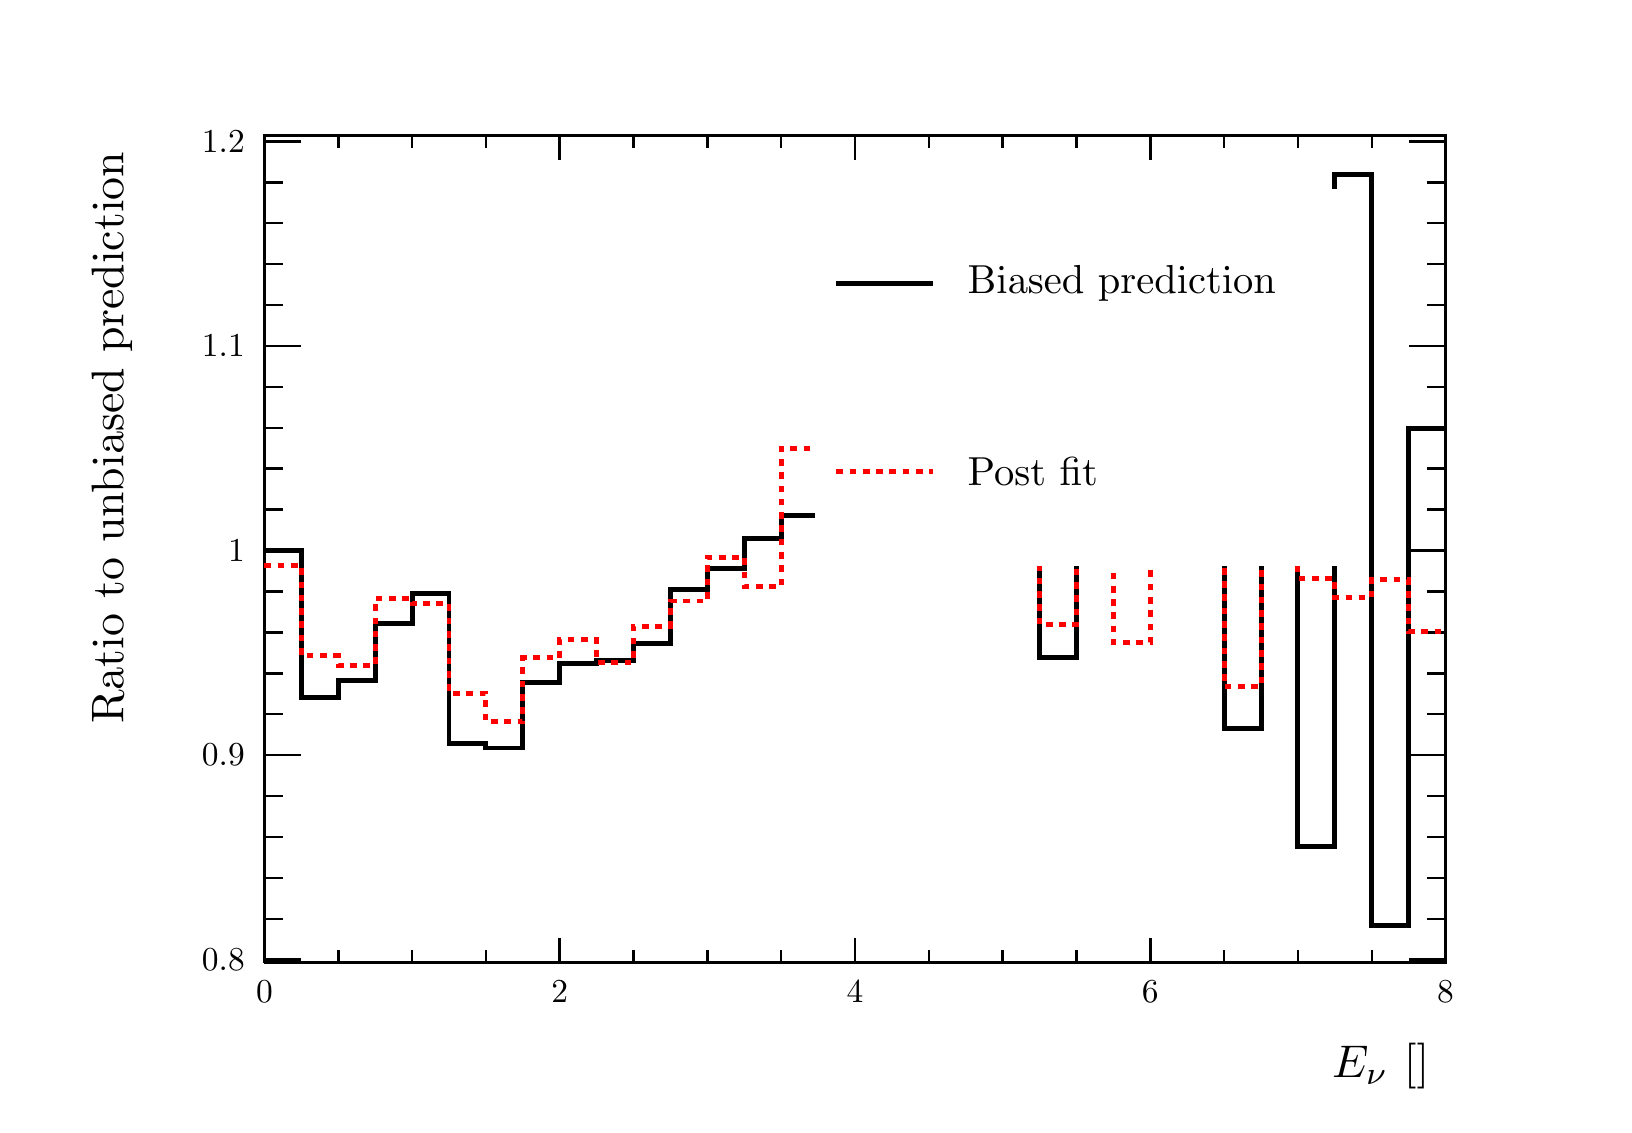
\begin{tikzpicture}
\pgfdeclareplotmark{cross} {
\pgfpathmoveto{\pgfpoint{-0.3\pgfplotmarksize}{\pgfplotmarksize}}
\pgfpathlineto{\pgfpoint{+0.3\pgfplotmarksize}{\pgfplotmarksize}}
\pgfpathlineto{\pgfpoint{+0.3\pgfplotmarksize}{0.3\pgfplotmarksize}}
\pgfpathlineto{\pgfpoint{+1\pgfplotmarksize}{0.3\pgfplotmarksize}}
\pgfpathlineto{\pgfpoint{+1\pgfplotmarksize}{-0.3\pgfplotmarksize}}
\pgfpathlineto{\pgfpoint{+0.3\pgfplotmarksize}{-0.3\pgfplotmarksize}}
\pgfpathlineto{\pgfpoint{+0.3\pgfplotmarksize}{-1.\pgfplotmarksize}}
\pgfpathlineto{\pgfpoint{-0.3\pgfplotmarksize}{-1.\pgfplotmarksize}}
\pgfpathlineto{\pgfpoint{-0.3\pgfplotmarksize}{-0.3\pgfplotmarksize}}
\pgfpathlineto{\pgfpoint{-1.\pgfplotmarksize}{-0.3\pgfplotmarksize}}
\pgfpathlineto{\pgfpoint{-1.\pgfplotmarksize}{0.3\pgfplotmarksize}}
\pgfpathlineto{\pgfpoint{-0.3\pgfplotmarksize}{0.3\pgfplotmarksize}}
\pgfpathclose
\pgfusepathqstroke
}
\pgfdeclareplotmark{cross*} {
\pgfpathmoveto{\pgfpoint{-0.3\pgfplotmarksize}{\pgfplotmarksize}}
\pgfpathlineto{\pgfpoint{+0.3\pgfplotmarksize}{\pgfplotmarksize}}
\pgfpathlineto{\pgfpoint{+0.3\pgfplotmarksize}{0.3\pgfplotmarksize}}
\pgfpathlineto{\pgfpoint{+1\pgfplotmarksize}{0.3\pgfplotmarksize}}
\pgfpathlineto{\pgfpoint{+1\pgfplotmarksize}{-0.3\pgfplotmarksize}}
\pgfpathlineto{\pgfpoint{+0.3\pgfplotmarksize}{-0.3\pgfplotmarksize}}
\pgfpathlineto{\pgfpoint{+0.3\pgfplotmarksize}{-1.\pgfplotmarksize}}
\pgfpathlineto{\pgfpoint{-0.3\pgfplotmarksize}{-1.\pgfplotmarksize}}
\pgfpathlineto{\pgfpoint{-0.3\pgfplotmarksize}{-0.3\pgfplotmarksize}}
\pgfpathlineto{\pgfpoint{-1.\pgfplotmarksize}{-0.3\pgfplotmarksize}}
\pgfpathlineto{\pgfpoint{-1.\pgfplotmarksize}{0.3\pgfplotmarksize}}
\pgfpathlineto{\pgfpoint{-0.3\pgfplotmarksize}{0.3\pgfplotmarksize}}
\pgfpathclose
\pgfusepathqfillstroke
}
\pgfdeclareplotmark{newstar} {
\pgfpathmoveto{\pgfqpoint{0pt}{\pgfplotmarksize}}
\pgfpathlineto{\pgfqpointpolar{44}{0.5\pgfplotmarksize}}
\pgfpathlineto{\pgfqpointpolar{18}{\pgfplotmarksize}}
\pgfpathlineto{\pgfqpointpolar{-20}{0.5\pgfplotmarksize}}
\pgfpathlineto{\pgfqpointpolar{-54}{\pgfplotmarksize}}
\pgfpathlineto{\pgfqpointpolar{-90}{0.5\pgfplotmarksize}}
\pgfpathlineto{\pgfqpointpolar{234}{\pgfplotmarksize}}
\pgfpathlineto{\pgfqpointpolar{198}{0.5\pgfplotmarksize}}
\pgfpathlineto{\pgfqpointpolar{162}{\pgfplotmarksize}}
\pgfpathlineto{\pgfqpointpolar{134}{0.5\pgfplotmarksize}}
\pgfpathclose
\pgfusepathqstroke
}
\pgfdeclareplotmark{newstar*} {
\pgfpathmoveto{\pgfqpoint{0pt}{\pgfplotmarksize}}
\pgfpathlineto{\pgfqpointpolar{44}{0.5\pgfplotmarksize}}
\pgfpathlineto{\pgfqpointpolar{18}{\pgfplotmarksize}}
\pgfpathlineto{\pgfqpointpolar{-20}{0.5\pgfplotmarksize}}
\pgfpathlineto{\pgfqpointpolar{-54}{\pgfplotmarksize}}
\pgfpathlineto{\pgfqpointpolar{-90}{0.5\pgfplotmarksize}}
\pgfpathlineto{\pgfqpointpolar{234}{\pgfplotmarksize}}
\pgfpathlineto{\pgfqpointpolar{198}{0.5\pgfplotmarksize}}
\pgfpathlineto{\pgfqpointpolar{162}{\pgfplotmarksize}}
\pgfpathlineto{\pgfqpointpolar{134}{0.5\pgfplotmarksize}}
\pgfpathclose
\pgfusepathqfillstroke
}
\definecolor{c}{rgb}{1,1,1};
\draw [color=c, fill=c] (0,0) rectangle (20,13.639);
\draw [color=c, fill=c] (3,1.77307) rectangle (18,12.2751);
\definecolor{c}{rgb}{0,0,0};
\draw [c,line width=0.9] (3,1.77307) -- (3,12.2751) -- (18,12.2751) -- (18,1.77307) -- (3,1.77307);
\definecolor{c}{rgb}{1,1,1};
\draw [color=c, fill=c] (3,1.77307) rectangle (18,12.2751);
\definecolor{c}{rgb}{0,0,0};
\draw [c,line width=0.9] (3,1.77307) -- (3,12.2751) -- (18,12.2751) -- (18,1.77307) -- (3,1.77307);
\draw [c,line width=1.8] (3,7.00538) -- (3.46875,7.00538) -- (3.46875,5.13675) -- (3.9375,5.13675) -- (3.9375,5.35275) -- (4.40625,5.35275) -- (4.40625,6.08102) -- (4.875,6.08102) -- (4.875,6.46115) -- (5.34375,6.46115) -- (5.34375,4.55299) --
 (5.8125,4.55299) -- (5.8125,4.49783) -- (6.28125,4.49783) -- (6.28125,5.32687) -- (6.75,5.32687) -- (6.75,5.56479) -- (7.21875,5.56479) -- (7.21875,5.60452) -- (7.6875,5.60452) -- (7.6875,5.82219) -- (8.15625,5.82219) -- (8.15625,6.5084) --
 (8.625,6.5084) -- (8.625,6.77341) -- (9.09375,6.77341) -- (9.09375,7.15418) -- (9.5625,7.15418) -- (9.5625,7.4504) -- (10.0312,7.4504) -- (10.0312,8.24554) -- (10.5,8.24554) -- (10.5,8.1855) -- (10.9688,8.1855) -- (10.9688,8.99686) --
 (11.4375,8.99686) -- (11.4375,8.75433) -- (11.9062,8.75433) -- (11.9062,9.75042) -- (12.375,9.75042) -- (12.375,7.79445) -- (12.8438,7.79445) -- (12.8438,5.64127) -- (13.3125,5.64127) -- (13.3125,9.28265) -- (13.7812,9.28265) -- (13.7812,8.53473) --
 (14.25,8.53473) -- (14.25,7.13) -- (14.7188,7.13) -- (14.7188,9.57608) -- (15.1875,9.57608) -- (15.1875,4.74636) -- (15.6562,4.74636) -- (15.6562,9.61079) -- (16.125,9.61079) -- (16.125,3.25258) -- (16.5938,3.25258) -- (16.5938,11.775) --
 (17.0625,11.775) -- (17.0625,2.24935) -- (17.5312,2.24935) -- (17.5312,8.55858) -- (18,8.55858);
\draw [c,line width=0.9] (3,1.77307) -- (18,1.77307);
\draw [c,line width=0.9] (3,2.07994) -- (3,1.77307);
\draw [c,line width=0.9] (3.9375,1.9265) -- (3.9375,1.77307);
\draw [c,line width=0.9] (4.875,1.9265) -- (4.875,1.77307);
\draw [c,line width=0.9] (5.8125,1.9265) -- (5.8125,1.77307);
\draw [c,line width=0.9] (6.75,2.07994) -- (6.75,1.77307);
\draw [c,line width=0.9] (7.6875,1.9265) -- (7.6875,1.77307);
\draw [c,line width=0.9] (8.625,1.9265) -- (8.625,1.77307);
\draw [c,line width=0.9] (9.5625,1.9265) -- (9.5625,1.77307);
\draw [c,line width=0.9] (10.5,2.07994) -- (10.5,1.77307);
\draw [c,line width=0.9] (11.4375,1.9265) -- (11.4375,1.77307);
\draw [c,line width=0.9] (12.375,1.9265) -- (12.375,1.77307);
\draw [c,line width=0.9] (13.3125,1.9265) -- (13.3125,1.77307);
\draw [c,line width=0.9] (14.25,2.07994) -- (14.25,1.77307);
\draw [c,line width=0.9] (15.1875,1.9265) -- (15.1875,1.77307);
\draw [c,line width=0.9] (16.125,1.9265) -- (16.125,1.77307);
\draw [c,line width=0.9] (17.0625,1.9265) -- (17.0625,1.77307);
\draw [c,line width=0.9] (18,2.07994) -- (18,1.77307);
\draw [anchor=base] (3,1.26842) node[scale=1.20912, color=c, rotate=0]{0};
\draw [anchor=base] (6.75,1.26842) node[scale=1.20912, color=c, rotate=0]{2};
\draw [anchor=base] (10.5,1.26842) node[scale=1.20912, color=c, rotate=0]{4};
\draw [anchor=base] (14.25,1.26842) node[scale=1.20912, color=c, rotate=0]{6};
\draw [anchor=base] (18,1.26842) node[scale=1.20912, color=c, rotate=0]{8};
\draw [anchor= east] (18,0.452814) node[scale=1.65459, color=c, rotate=0]{$E_{\nu}$ [\si{\GeV}]};
\draw [c,line width=0.9] (3,12.2751) -- (18,12.2751);
\draw [c,line width=0.9] (3,11.9682) -- (3,12.2751);
\draw [c,line width=0.9] (3.9375,12.1216) -- (3.9375,12.2751);
\draw [c,line width=0.9] (4.875,12.1216) -- (4.875,12.2751);
\draw [c,line width=0.9] (5.8125,12.1216) -- (5.8125,12.2751);
\draw [c,line width=0.9] (6.75,11.9682) -- (6.75,12.2751);
\draw [c,line width=0.9] (7.6875,12.1216) -- (7.6875,12.2751);
\draw [c,line width=0.9] (8.625,12.1216) -- (8.625,12.2751);
\draw [c,line width=0.9] (9.5625,12.1216) -- (9.5625,12.2751);
\draw [c,line width=0.9] (10.5,11.9682) -- (10.5,12.2751);
\draw [c,line width=0.9] (11.4375,12.1216) -- (11.4375,12.2751);
\draw [c,line width=0.9] (12.375,12.1216) -- (12.375,12.2751);
\draw [c,line width=0.9] (13.3125,12.1216) -- (13.3125,12.2751);
\draw [c,line width=0.9] (14.25,11.9682) -- (14.25,12.2751);
\draw [c,line width=0.9] (15.1875,12.1216) -- (15.1875,12.2751);
\draw [c,line width=0.9] (16.125,12.1216) -- (16.125,12.2751);
\draw [c,line width=0.9] (17.0625,12.1216) -- (17.0625,12.2751);
\draw [c,line width=0.9] (18,11.9682) -- (18,12.2751);
\draw [c,line width=0.9] (3,1.77307) -- (3,12.2751);
\draw [c,line width=0.9] (3.462,1.80939) -- (3,1.80939);
\draw [c,line width=0.9] (3.231,2.32899) -- (3,2.32899);
\draw [c,line width=0.9] (3.231,2.84859) -- (3,2.84859);
\draw [c,line width=0.9] (3.231,3.36819) -- (3,3.36819);
\draw [c,line width=0.9] (3.231,3.88778) -- (3,3.88778);
\draw [c,line width=0.9] (3.462,4.40738) -- (3,4.40738);
\draw [c,line width=0.9] (3.231,4.92698) -- (3,4.92698);
\draw [c,line width=0.9] (3.231,5.44658) -- (3,5.44658);
\draw [c,line width=0.9] (3.231,5.96618) -- (3,5.96618);
\draw [c,line width=0.9] (3.231,6.48578) -- (3,6.48578);
\draw [c,line width=0.9] (3.462,7.00538) -- (3,7.00538);
\draw [c,line width=0.9] (3.231,7.52498) -- (3,7.52498);
\draw [c,line width=0.9] (3.231,8.04458) -- (3,8.04458);
\draw [c,line width=0.9] (3.231,8.56418) -- (3,8.56418);
\draw [c,line width=0.9] (3.231,9.08378) -- (3,9.08378);
\draw [c,line width=0.9] (3.462,9.60338) -- (3,9.60338);
\draw [c,line width=0.9] (3.231,10.123) -- (3,10.123);
\draw [c,line width=0.9] (3.231,10.6426) -- (3,10.6426);
\draw [c,line width=0.9] (3.231,11.1622) -- (3,11.1622);
\draw [c,line width=0.9] (3.231,11.6818) -- (3,11.6818);
\draw [c,line width=0.9] (3.462,12.2014) -- (3,12.2014);
\draw [c,line width=0.9] (3.462,1.80939) -- (3,1.80939);
\draw [c,line width=0.9] (3.462,12.2014) -- (3,12.2014);
\draw [anchor= east] (2.9,1.80939) node[scale=1.20912, color=c, rotate=0]{0.8};
\draw [anchor= east] (2.9,4.40738) node[scale=1.20912, color=c, rotate=0]{0.9};
\draw [anchor= east] (2.9,7.00538) node[scale=1.20912, color=c, rotate=0]{1};
\draw [anchor= east] (2.9,9.60338) node[scale=1.20912, color=c, rotate=0]{1.1};
\draw [anchor= east] (2.9,12.2014) node[scale=1.20912, color=c, rotate=0]{1.2};
\draw [anchor= east] (1.064,12.2751) node[scale=1.65459, color=c, rotate=90]{Ratio to unbiased prediction};
\draw [c,line width=0.9] (18,1.77307) -- (18,12.2751);
\draw [c,line width=0.9] (17.538,1.80939) -- (18,1.80939);
\draw [c,line width=0.9] (17.769,2.32899) -- (18,2.32899);
\draw [c,line width=0.9] (17.769,2.84859) -- (18,2.84859);
\draw [c,line width=0.9] (17.769,3.36819) -- (18,3.36819);
\draw [c,line width=0.9] (17.769,3.88778) -- (18,3.88778);
\draw [c,line width=0.9] (17.538,4.40738) -- (18,4.40738);
\draw [c,line width=0.9] (17.769,4.92698) -- (18,4.92698);
\draw [c,line width=0.9] (17.769,5.44658) -- (18,5.44658);
\draw [c,line width=0.9] (17.769,5.96618) -- (18,5.96618);
\draw [c,line width=0.9] (17.769,6.48578) -- (18,6.48578);
\draw [c,line width=0.9] (17.538,7.00538) -- (18,7.00538);
\draw [c,line width=0.9] (17.769,7.52498) -- (18,7.52498);
\draw [c,line width=0.9] (17.769,8.04458) -- (18,8.04458);
\draw [c,line width=0.9] (17.769,8.56418) -- (18,8.56418);
\draw [c,line width=0.9] (17.769,9.08378) -- (18,9.08378);
\draw [c,line width=0.9] (17.538,9.60338) -- (18,9.60338);
\draw [c,line width=0.9] (17.769,10.123) -- (18,10.123);
\draw [c,line width=0.9] (17.769,10.6426) -- (18,10.6426);
\draw [c,line width=0.9] (17.769,11.1622) -- (18,11.1622);
\draw [c,line width=0.9] (17.769,11.6818) -- (18,11.6818);
\draw [c,line width=0.9] (17.538,12.2014) -- (18,12.2014);
\draw [c,line width=0.9] (17.538,1.80939) -- (18,1.80939);
\draw [c,line width=0.9] (17.538,12.2014) -- (18,12.2014);
\definecolor{c}{rgb}{1,0,0};
\draw [c,dash pattern=on 2.40pt off 2.40pt ,line width=1.8] (3,6.81757) -- (3.46875,6.81757) -- (3.46875,5.66739) -- (3.9375,5.66739) -- (3.9375,5.54465) -- (4.40625,5.54465) -- (4.40625,6.40189) -- (4.875,6.40189) -- (4.875,6.33079) --
 (5.34375,6.33079) -- (5.34375,5.19243) -- (5.8125,5.19243) -- (5.8125,4.82963) -- (6.28125,4.82963) -- (6.28125,5.64282) -- (6.75,5.64282) -- (6.75,5.87818) -- (7.21875,5.87818) -- (7.21875,5.58931) -- (7.6875,5.58931) -- (7.6875,6.04633) --
 (8.15625,6.04633) -- (8.15625,6.3648) -- (8.625,6.3648) -- (8.625,6.92293) -- (9.09375,6.92293) -- (9.09375,6.54875) -- (9.5625,6.54875) -- (9.5625,8.30655) -- (10.0312,8.30655) -- (10.0312,7.65132) -- (10.5,7.65132) -- (10.5,8.3762) --
 (10.9688,8.3762) -- (10.9688,8.87183) -- (11.4375,8.87183) -- (11.4375,8.6821) -- (11.9062,8.6821) -- (11.9062,8.63701) -- (12.375,8.63701) -- (12.375,7.84487) -- (12.8438,7.84487) -- (12.8438,6.06569) -- (13.3125,6.06569) -- (13.3125,9.93151) --
 (13.7812,9.93151) -- (13.7812,5.83429) -- (14.25,5.83429) -- (14.25,8.95677) -- (14.7188,8.95677) -- (14.7188,7.515) -- (15.1875,7.515) -- (15.1875,5.27506) -- (15.6562,5.27506) -- (15.6562,7.77194) -- (16.125,7.77194) -- (16.125,6.6522) --
 (16.5938,6.6522) -- (16.5938,6.40441) -- (17.0625,6.40441) -- (17.0625,6.63673) -- (17.5312,6.63673) -- (17.5312,5.97654) -- (18,5.97654);
\definecolor{c}{rgb}{1,1,1};
\draw [color=c, fill=c] (10,6.81948) rectangle (17,11.5931);
\definecolor{c}{rgb}{0,0,0};
\draw [anchor= west] (11.75,10.3997) node[scale=1.46368, color=c, rotate=0]{Biased prediction};
\draw [c,line width=1.8] (10.2625,10.3997) -- (11.4875,10.3997);
\draw [anchor= west] (11.75,8.01289) node[scale=1.46368, color=c, rotate=0]{Post fit};
\definecolor{c}{rgb}{1,0,0};
\draw [c,dash pattern=on 2.40pt off 2.40pt ,line width=1.8] (10.2625,8.01289) -- (11.4875,8.01289);
\end{tikzpicture}
